%%%%%%%%%%%%%%%%%%%%%%%%%%%%%%%%%%%%%%%%%%%%%%%%%%%%%%%%%%%%%%%%%%% 
%                                                                 %
%                             Animation                           %
%                                                                 %
%%%%%%%%%%%%%%%%%%%%%%%%%%%%%%%%%%%%%%%%%%%%%%%%%%%%%%%%%%%%%%%%%%% 
 
\chapter{SIMULATION METHOD FOR A JUMPING MOTION}
\label{chapter:animation}
In this chapter we describe our method for simulating a character.  We begin by describing the motion, breaking it into stages in Section \ref{section:motion_desc}.  In Section \ref{section:setup_inputs} we then describe the setup of the problem and inputs to our simulation.  As part of our description of the inputs to the simulation, we describe the representation of a skeleton in detail in Section \ref{subsection:skel_joints} as well as the other user specified constants in Section \ref{subsection:user_constants}.  Following the problem setup, we describe our inverse kinematics solver in Section \ref{section:ik}, and balancing of the character in Section \ref{section:com}.  We then describe two methods of simulation: the first using torque on a joint to describe the motion in Section \ref{section:torque} and the second using energy of the muscles to describe the motion in Section \ref{section:energy}.  The stages of jumping are described for each of these calculation paths.

\section{Overview of a Jumping Motion}
\label{section:motion_desc}
Jumping is the acceleration of a character's center of mass upward.  Acceleration is applied in excess and in opposition to gravity, resulting in the character breaking contact with the ground and traveling a short distance before contact is re-established.  This acceleration results due to the character pushing against the ground, first bending to create space and lengthen muscles, then extending, contracting the muscles.

Jumping motions can be divided into several stages.  First is the lead-up or wind-up stage in which the character flexes, preparing their muscles for contraction and providing space for their body to extend.  This takes the form of a slight crouch.  Next comes the thrust stage, in which the character extends and exerts a force against the ground to accelerate upward.  The character pushes against the floor with their feet, the contractions of the muscles causing joints to unbend and as a result displace the character's center of mass causing work to be done.  This extension and resulting thrust is caused by the contraction of muscles, which produce torques on the skeleton.

Once the character has broken contact with the ground, they travel through the air, their velocity decreasing steadily due to gravity, air resistance, and other forces until they eventually land.  Once they regain contact with the ground, the character absorbs or disperses the kinetic energy of their jump.

We attempted two main approaches to producing a jump motion through muscle simulation.  The first method focused heavily on the torques produced by the muscles, but ultimately failed to converge, and consistently moved towards a solution that appears incorrect, where the character begins to lean towards the right.  These calculated values were also extremely small as compared to the calculated required values, despite repetitions of the math derivation and careful debugging.  The second method focused on the kinetic energy and performed calculations to match the energy of the muscles, which simplifies the movement and produced a successful simulation.

\section{Model Initialization and Setup}
\label{section:setup_inputs}
\subsection{Creation of the Model and Rig}
\label{subsection:model_rig}


%TODO make the images the same level of zoom
\begin{figure}[htp]
	\centering
	\begin{subfigure}[b]{0.41\textwidth}
		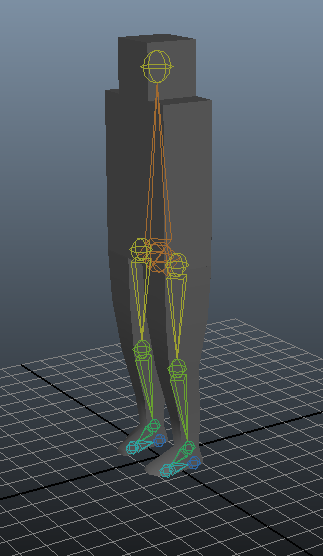
\includegraphics[width=\textwidth]{images/simpleSkeleton2Screen1Cropped.png}
	\end{subfigure}
	\begin{subfigure}[b]{0.3\textwidth}
		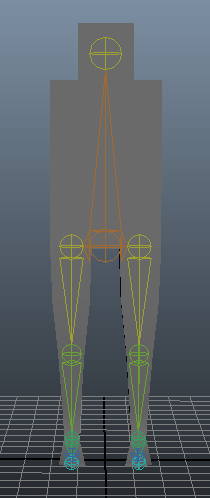
\includegraphics[width=\textwidth]{images/simpleSkeleton2Screen2Cropped.png}
	\end{subfigure}
	\caption[Example of Rigged 3D Character Model]{Above is an example of a character model in \maya{}, the character used for our simulation.  The character skin or mesh is shown in gray, with a rig shown in multicolor.  While it is visualized as a series of spherical joints with connecting solids, the rig itself does not have a visual component in practice.  The rig acts as a skeleton, deforming the mesh of the character model to make animation easier.  Additional tools such as user-specified skeletal controls and inverse kinematic handles can be used to further simplify the creation of animations for artists.  While these tools simplify movement of the model, the artist still must position each joint for each frame of the animation, which is then stored for later playback.  This rig contains 11 bones and 12 joints: a pelvis, two hips, two knees, two ankles, two toes, two heels, and one head.  In this visual, orange bones and joints are connected directly to the root, the pelvis, yellow are the first level of the tree, green the second, light blue the third, and dark blue the fourth level of the tree.}
	\label{fig:rig_character}
\end{figure}

The character in our system consists of a mesh, a skeleton or \emph{rig}, and a controller which has itself several sub-components.  First we constructed a mesh, a 3D visual representation of our character.  Our mesh is a simple, blocky humanoid, lacking arms in order to focus on the motion of the lower body.  A more complex human character, or non-human bipedal characters could be substituted.  This mesh consists of vertices, which each have a position as well as other information not relevant to our simulation such as normal and texture coordinate, which are used by \unity{} for displaying the mesh.  This mesh can also be referred to as a character model, but in the context of this simulation we will refer to it as the mesh.  Three vertices form a triangular face, though these are often created as quadrilaterals by the artist as the topology of the model can be simpler to work with due to the grid patterns formed as compared to triangular meshes.  In the case of quad meshes, the mesh is often treated as a triangle mesh by the game engine or renderer, with each quad split into two triangles.

Our mesh was created using \maya{}, positioning the vertices in groups or individually, using several rectangular prisms as a base.  Using the edge loop tool, more vertices were inserted, with loops of edges circling the torso and legs to produce the final shape.  This mesh was then rigged, meaning a skeleton was added.  As described in further detail in section \ref{subsection:skel_joints}, joints were positioned individually relative to the mesh, attempting to mimic the positioning of joints in the human skeleton.  The connections were made simply, with each joint acting as a ball and socket joint, meaning that constraints needed to be specified at a later stage to facilitate hinge joints such as the knee and ankle and that complex, multi-boned structures as found in the human foot and shin were simplified to a single bone connecting two joints.  The hierarchy of joints for the skeleton was rooted at the pelvis with three children: one leading to the upper body and one to each hip.  From there a single joint was used for the manipulation of the upper body, with separate joints for each hip, knee, ankle, toe, and heel.  Though there is no movement in the toe, placing a bone for the foot requires an end joint for the bone to connect to.

%TODO how do i talk about this with authority, there isn't really anything to cite there's just youtube videos and it's generally taught as such/discovered via industry
% found some articles, gamasutra especially
Joints are then associated with the mesh through weight painting, in which each vertex of the mesh is assigned a weight for each joint.  This weight designates if and how much a vertex transforms when a joint is moved.  Each vertex must be assigned a weight for each joint of the model.  Careful weight assignment is highly important as this determines the behavior of the character's ``skin'' when they move, affecting how the mesh twists or bends as well as which parts move with which bones.  The joints may then be used to manipulate the mesh to produce animations, with each key frame in an animation storing information about each joint instead of each vertex. %\cite{gamasutra_char_anim}

\subsection{Environmental and Jump Constants}
\label{subsection:user_constants}
% specified constants
% gravity
% air time
% windup time
% error allowance (between calculated skeleton values and desired)
% drag
% jumping policy (not implemented)
% Windup PD k values
% Balance PD k values
% muscle values foreach muscle:
%	k (linear spring constant)
%	anchor joints (for our simulation, 2)
% 	center joint
%   [0,1] scale to indicate muscle anchor position (0 is closer to center joint, 1 is closer to end joint)
%   bone width
% calculated values
Within the controller there are a number of constants the user can specify, outside of the character itself.  These specify constants for the simulation environment as well as some constants describing the animation to be produced.  Our only environmental constant is gravity, which we specify as -10 $\frac{m}{s^2}$, where the negative indicates the downward direction.  Other constants include the air time, windup time, error allowance, and constants for the PID controllers which specify a multiplicative factor for the proportional, integral, and derivative components of each PID controller.

The times indicate how much time the character is expected to spend in the air and winding up for the jump.  Air time in our case consists of the portion of the animation where the character's feet are not in contact with the ground plane.  Windup time refers to the time in which the character has their feet on the ground and is in the process of accelerating their mass upwards as the initial takeoff portion of the jump.  A long windup time gives a very slow, exaggerated jumping motion while a short windup gives a very rapid, clipped motion.  While we allow the user to specify any time for both air and windup, in practice there is a limited range of values that are possible for the character.  Values outside of the reasonable range produce indeterminate or strange behaviors in the simulation, such as either failing to find a muscle load that can feasibly produce the jump or attempting to produce the jump and failing partway.

%TODO table of values from testing excel sheet showing why it fails
\begin{table}[ht]
	\centering
	\begin{tabular}{| c | c | c | c |}
	\hline
	Input $\mathbf{t_a}$ ($s$) & Calculated $\mathbf{a}$ ($\frac{m}{s^2}$) & Calculated $\mathbf{v_{0}}$ ($m$) \\ \hline
	0.1 & (0, 2.5,  50)    & (0, 0.5, 10)   \\ \hline
	0.2 & (0, 5,    25)    & (0, 1,   5)    \\ \hline
	0.3 & (0, 7.5,  16.67) & (0, 1.5, 3.33) \\ \hline
	0.4 & (0, 10,   12.5)  & (0, 2,   2.5)  \\ \hline
	0.5 & (0, 12.5, 10)    & (0, 2.5, 2)    \\ \hline
	0.6 & (0, 15,   8.33)  & (0, 3,   1.67) \\ \hline
	0.7 & (0, 17.5, 7.14)  & (0, 3.5, 1.43) \\ \hline
	0.8 & (0, 20,   6.25)  & (0, 4,   1.25) \\ \hline
	0.9 & (0, 22.5, 5.56)  & (0, 4.5, 1.11) \\ \hline
	1.0 & (0, 25,   5)     & (0, 5,   1)    \\ \hline
	1.1 & (0, 27.5, 4.55)  & (0, 5.5, 0.91) \\ \hline
	1.2 & (0, 30,   4.17)  & (0, 6,   0.83) \\ \hline
	1.3 & (0, 32.5, 3.85)  & (0, 6.5, 0.77) \\ \hline
	1.4 & (0, 35,   3.57)  & (0, 7,   0.71) \\ \hline
	1.5 & (0, 37.5, 3.33)  & (0, 7.5, 0.67) \\ \hline
\end{tabular}
	\caption{Values for calculated necessary velocity given air and windup times for a skeleton with muscle k values around 20000. This table shows calculated necessary acceleration and velocity for the character given constant jump displacement of $x - x_0 = (0, 0, 1)m$, gravity $g=(0, -10, 0)\frac{m}{s^2}$, and windup time $t_w = 0.2s$, where windup time refers to the amount of time the force of the jump is applied to the character. Values are calculated with variable desired air time $t_a$ in range $[0.1, 1.5]s$ with a step of $0.1s$, where $v_0$ is the velocity when the character leaves the ground, and $a$ is acceleration required to reach $v_0$ from rest.}
\end{table}

Error allowance in our simulation is a widely used value indicating a percent error tolerance.  This tolerance is used for determining the allowable difference between the desired values of either resultant linear acceleration and desired acceleration for the torque based simulation, or calculated kinetic energy and total elastic energy for the energy based simulation.  The allowable difference is used for choosing samples and determining if the character has satisfied either the energy or acceleration requirements to complete the windup stage.  The same error allowance is also used to determine if the limb usage is greater than a minimum to complete the windup stage, which is used to force a degree of bend in extreme cases, where very little bend is required as the muscles are extremely strong or the jump distance is very small.  This minimum is applied to compensate for the contraction rates of muscles, which would require a higher degree of bend than our muscle model does, leading to a more realistic simulation.  We use an $\epsilon=0.05$ for calculating our percent error allowance, and a separate, floating point epsilon of 0.001 for comparison of floating point numbers.  Below is an example of the inequality using the error allowance.  

\[
	E_{kinetic} - E_{elastic} \le \epsilon E_{kinetic}
\]

\begin{table}[ht]
	\centering
	\begin{tabular}{|c|c|c|}
		\hline
		& Windup & Balance \\ \hline
		$k_p$ & 0.25 & 1 \\ \hline
		$k_i$ & 0 & 0 \\ \hline
		$k_d$ & 0.25 & 1 \\ \hline
	\end{tabular}
	\caption[PID controller constants for our simulation]{Above are the proportional ($k_p$), integral ($k_i$), and derivative ($k_d$) constants for the two PID controllers used in our simulations.  One controller handles feedback control of the bend of the character, working with the error between the required output of the muscles and the desired output while the second handles the balance of the character, minimizing the distance of the character's center of mass from the center of the character's supporting polygon through feedback control.  These constants act as a weight on the different components of the controller, adjusting the rate of control and the rate of control relative to the error, constant error, and change in error through the proportional, integral, and derivative components respectively.}
\end{table}

Lastly, we utilize proportional-integral-derivative (PID) controllers, which require 3 constants for each controller.  A PID controller modifies an input based on error in 3 ways: proportional to the error, proportional to the integral of the error, and proportional to the derivative of the error \cite{pid}.  This allows changes to the system to have gains directly related to the error through the proportional component, eliminate steady-state error with the integral component, and to adjust gain with the derivative to improve stability of the changes.  Our system does not require an integral component, meaning our controllers are just PD controllers with their constant for I set to 0.  For our controllers, as we work in discrete frames, our controller calculation is as follows.
\[
	u(t) = k_p e(t) + k_i \displaystyle\sum_{\tau = 0}^t e(\tau) + k_d \left( e(t) - e(t-1) \right)
\]

%TODO example windup times with our chosen values

\subsection{Skeleton, Joints, and Muscles}
\label{subsection:skel_joints}

For the purposes of animation, a joint is an object with an associated position, associated transformation, a parent joint, and some number of child joints.  In the case of the root, the parent joint is absent and in the case of the end joints such as tips of the fingers there are no child joints.  Each child joint is connected to the parent by a rigid bone, which protrudes from the parent at a given resting angle.  These joints are structured in a tree, as the parent and child joints imply, with the root of the tree at the pelvis.  This tree serves as a hierarchy for transformations.  Figure \ref{fig:rig_character} shows the skeleton for our character.

Joints are associated with a set of vertices from the mesh to be animated.  Each of these may be associated with multiple joints, and are assigned a weight for each joint which acts as a scale factor for the transformations performed on the vertex.  When a joint is transformed, the transformation is propagated to the children, with the parent as the origin of the child node's coordinate system.

In addition to the animation-related functions, joints in our system handle a number of other functions and values.  Each joint keeps track of its constraints on rotation.  Rotations are performed axis-angle, that is a rotation is specified as a rotation $\theta$ degrees around an arbitrary axis $\vec{e} \in \mathbb{R}^3$. This makes the constraints somewhat more complicated as compared to euler angles in exchange for simpler, rotations.  

Constraints, however, are specified through euler angles: pitch, roll, and yaw.  These correspond to a rotation about the x, z, and y axes respectively in \unity{}'s coordinate system.  When rotating using a traditional rotation matrix through Euler angles, constraints simply prevent any of the angles from exceeding the bounds.  The other issue was how to constrain a joint when rotation about a certain axis was fully prohibited, such as the knee joint which can only rotate about the x-axis.  To constrain the axis-angle rotation thus, simply zero the undesirable component of the vector.  Constraining the axis-angle rotation to a region with degree minima and maxima for rotations around the x, y, and z axes requires definition and constraint to the region of a sphere the rotation constraints covers.  Instead of solving this complex problem, we instead clamp the euler angles to their constrained regions after each rotation, forcing the controller and the inverse kinematics solver to operate within the region and thus reducing the possible solutions for each to only those solutions within the region.

Along with constraints, each joint tracks a weight, which allows distribution of weight over the body.  This distribution affected the torque simulation heavily as the torque of each joint resulted in a different angular momentum depending on the mass distribution.  The energy simulation considered the character as a rigid body, not considering the changes occurring due to weight distribution except for balance issues and the effects on the muscles as described shortly.  Joints also provide functions for calculating the direction to the next joint for muscle calculations, and a utility function for returning to a resting position.

\begin{figure}[ht]
	\centering
	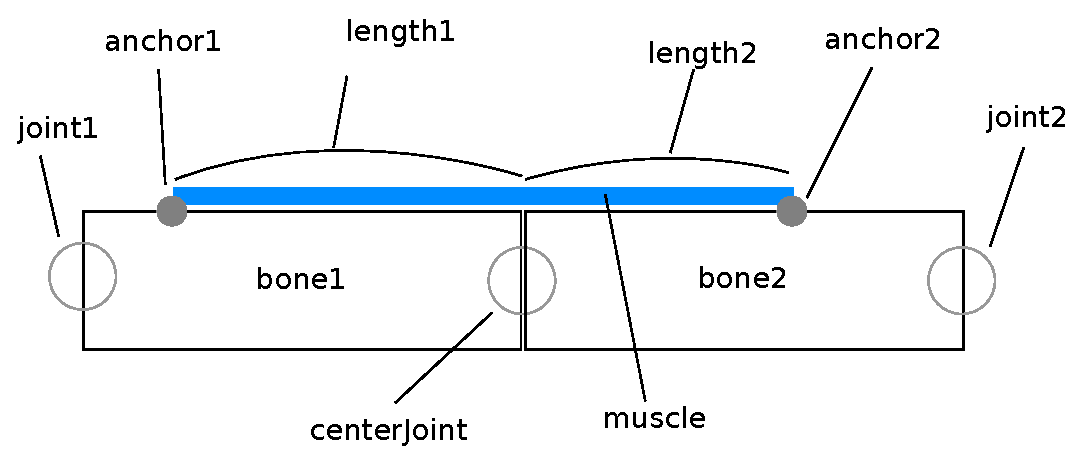
\includegraphics[width=10cm]{images/spring_calc/spring_anchors.eps}
	\caption[Diagram of muscle definition showing anchor points and joints used for specification]{Pictured is a diagram of how a muscle is defined.  Three joints are used: joint1, joint2, and centerJoint, where centerJoint is the joint the muscle crosses.  The center of rotation for the joint is conceptualized as at the edge of the bone as shown above, with the movement modeled after connecting a pair of blocks with a rubber band, though the joint is positioned at the center of the bone.  As the bone used to calculate the muscle forces is only loosely related to the bone of the character's rig, this does not introduce errors as the model is kept internally consistent with only the angle and relative positions of the joints used for the calculation.}
	\label{fig:muscle_anchors}
\end{figure}

Several joints form a muscle.  Though any number of joints is possible, our muscles only utilize 3 joints each.  These joints serve as anchor points for the muscles, with each anchor point specified as a number in $[0, 1]$ between the center joint, i.e. the joint the muscle crosses, and the other joint the bone connects to.  In this way three joints describe the path of a muscle in our system.  The muscle itself is a linear spring, obeying Hooke's law.  This gives force ($F$) and elastic energy ($E_{elastic}$) as
\begin{align*}
	F &= -ks \\
	E &= \frac{1}{2} k s^2
\end{align*}
where $k$ is the spring constant for the muscle and $s$ is the displacement of the spring.  The negation of $k$ in the force calculation indicates the force restores the spring to rest.  These anchor points and the method of muscle specification are shown in Figure \ref{fig:muscle_anchors}.  While the muscle in Figure \ref{fig:muscle_anchors} is at rest when the joint is straightened, the rest angle can be specified arbitrarily to handle, for example, the right angles of the muscles crossing the ankles and hips, as the hip muscles span from pelvis to hip to knee.

Intuitively, this models the bones as blocks, with a spring representing a combination of the muscle and tendons connecting the blocks.  When the joint rotates, the spring necessarily stretches, producing a restoring force attempting to retract the spring to its initial length.  This then produces a torque on the blocks involved, causing a torque on the blocks at the joint.  As one block is more strongly anchored than the other, i.e. the part of the joint chain closer to the foot and thus the ground is less able to move freely as more of the character's weight is resting on it, one bone rotates about the joint center.  The user is free to then restrict this motion further by specifying ranges of motion for the joint to mimic human capabilities.

Considering a muscle as a spring models a muscle at maximum activation.  A relaxed muscle has very little contractual or restoring force, and thus a low value for $k$, while a flexed muscle has a large $k$.  While the muscle model could take muscle activation level into account, we chose the simpler system, allowing the user to specify $k$ for their particular case.  This gives more control for the animation, but also allows for more errors and issues.  The results with poorly chosen $k$ values resemble the results with poorly chosen times.

\begin{figure}[ht]
	\centering
	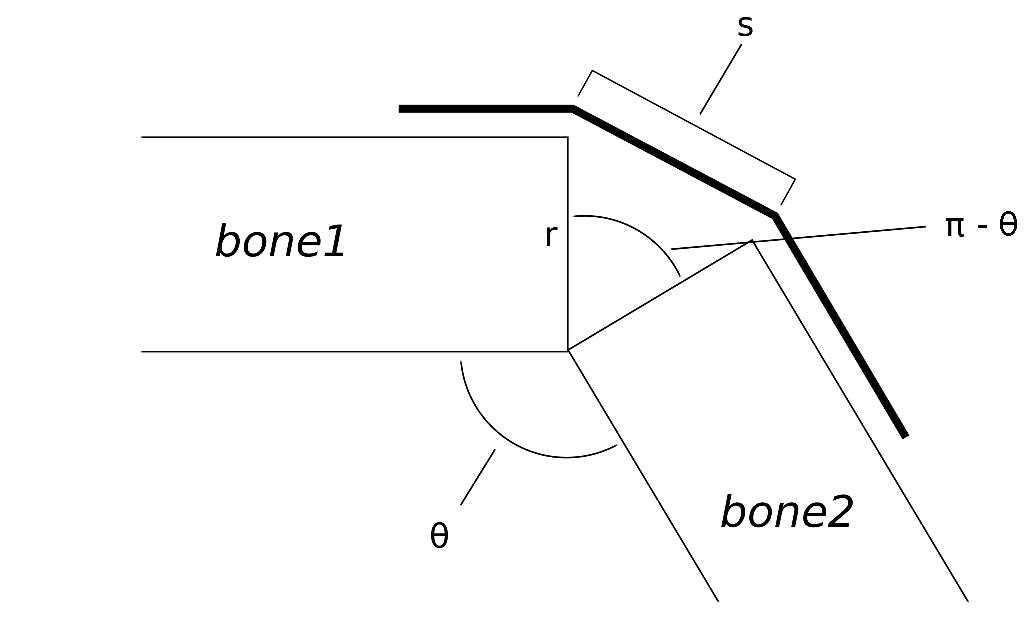
\includegraphics[width=10cm]{images/spring_calc/angle_diag.eps}
	\caption[Diagram of spring displacement calculation]{Above is a visual representation of the angles used to calculate the spring displacement.  The angle of the joint, $\theta$, is used to calculate the displacement $s$ using the bone width $r$ and the law of sines.  Angles for the joint are restricted to the range $(0, \pi)$, with values outside of this range producing an undefined $s$.  As a bend in the reverse direction, considering rotation about each axis separately, produces an equivalent situation, the absolute value of the angle is used and the equivalent angle within the range is found.  For negative angles, an adjustment is made in the direction to account for the difference in the direction of the forces produced after calculating the displacement, reversing the sign on the resulting torque or altering the direction of acceleration for the energy calculation.}
	\label{fig:angleDiag}
\end{figure}

Along with the $s$ values, a muscle keeps track of its center joint, anchor joints, and the bone width.  A muscle has two anchor points and crosses the center joint.  The positions of the anchors are specified as values in the range $[0,1]$ along the bone between the center joint and the anchors.  Bones are considered to be rectangular prisms with a square cross-section, with a width $r$ specified by the user.  Spring displacement can then be calculated directly from the angle of the joint using these constants and our assumptions as illustrated in Figure \ref{fig:forceCalc} with the equation below derived from the law of sines:
\[ 
	s = \dfrac{r\sin\left(\pi - \theta \right)}{\sin\frac{\theta}{2}}
\]
We derive this equation by calculating the supplementary angle, opposite the spring displacement.  This angle can therefore be expressed as $\pi - \theta$. The sum of the remaining angles of the triangle formed by the spring displacement and bone ends can then be expressed as $\frac{\theta}{2}$.  These angles are shown in Figure \ref{fig:angleDiag}. We assume uniform bone width, which allows a simpler calculation of the angles.

For debugging purposes and for calculating the extension of the limb we have each muscle calculate its utilization, giving a value in $[0,1]$.  Utilization is a number used to determine if a muscle is being stretched and producing a force, indicating if the muscle is too weak or is simply not being used by the simulation.  This utilization is calculated as the dot product of the normalized vectors between the center joint and the anchor points.  The value is then scaled from $[-1, 1]$ to $[0,1]$ by adding 1 and dividing by 2.  A modification to this function is required for joints at rest at angles other than 0 or $\pi$ radians, instead using a comparison to the stored rest angle of the joint.

As an additional debugging tool and method of determining the expected ranges of values, we calculated the values in Table \ref{tab:force_est}.  By testing different ranges of values and comparing with some expected values, we determined empirically a range of values that should produce ``normal'' human simulation, i.e. expected strength values required for several different heights given body mass and proportions.  An military study of male aviators in 1988 provided information on mass, mass distribution, and the dimensions of different body sections.  Range of motion data was obtained from Boone and Azen who compared clinical measurements with estimations in the handbook of The American Academy of Orthopaedic Surgeons as a reference \cite{Boone756}.


\section{Center of Mass and Maintaining Balance}
\label{section:com}
The center of mass (CoM) is calculated as the centroid of the character.  More specifically, joint positions are averaged, with a weight assigned to each joint based on the weight of the limb associated.  The CoM must be recalculated with each update to the character's pose as the shift in weight changes the position.

Using the calculated CoM, the balance of the character can be determined by the position of the CoM relative to the supporting polygon of the character.  The supporting polygon is a polygon determined by the points of contact of the character with the ground or other supports which provide a normal force to counteract gravity and other external forces.  During the windup and thrust phases, the character maintains contact with the ground through their feet, with the outer edges of the feet forming two sides of a quad, a line between the two feet at the toes forming a third, and a line between the heels of the character forming the fourth side.  This polygon should be parallel to the ground plane, and is positioned at the bottom of the feet.  If the character's center of mass is over this supporting polygon, the character is balanced.

To quantify balance, the vector between the center of the supporting polygon and the position of the CoM is measured.  This vector is then projected into the same plane as the supporting polygon, giving a 2 dimensional error between where the CoM is currently and where it would need to be to be perfectly centered.  The PD controller then attempts to minimize the magnitude of this vector by moving in the prescribed direction while bending to achieve the desired force, constraining the number of solutions possible to provide the desired force.

% does the vertical distance have effect?  you're going to fall over more easily if you're on a stilt as opposed to crouching over your feet as the moment will be (bigger? is that bigger?).  the lever will be more able to move your weight easily

% upper body rebalancing
As the character bends for the windup and extends for thrusting, the character must rebalance with minimal change in flexion, i.e. height of the hips, in order to maintain the calculated load on the muscles.  For these cases, the upper body is used to rebalance.  The character bends forwards, backwards, left, and right to shift the weight of the upper body to offset the balance error created by the lower body pose.  This is performed using a PD controller, with the error input as the balance error as calculated above, and the output as the amount to rotate in each direction subject to skeletal constraints.

\section{Inverse Kinematic Solving for Ankle and Knee Position}
\label{section:ik}


As the skeleton is a hierarchy assumed to be rooted at the hip, a problem arises with applying rotations to joints.  To keep a character's feet rooted to the floor as is expected, positions must be solved for using inverse kinematics.  Given the desired position for the hip, and the desired position of the foot, we solve for the joint angles and positions of the knee and ankle.  Constraints are placed on each joint, limiting the range of motion to an expected range as well as limiting the axes about which each joint can rotate, preventing unnatural directions of motion.  These values are specified per joint and can be edited by the user to simulate varied levels of flexibility or alternate body shapes.

%TODO alternate body with digitigrade, Tauren or whatever from WoW, raptor style...
%TODO Further justification of why choosing this method instead of learning is that this is more user-tunable as opposed to a learning heavy model which doesn't allow as much user tuning

%\begin{table}[ht]
%	\centering
%	\caption[Table of joint constraints]{Joint angle constraint values used for each joint, with accompanying images of expected motion range.}
%	\label{tab:jointConstraints}
%\end{table}

\begin{figure}[ht]
	\centering
	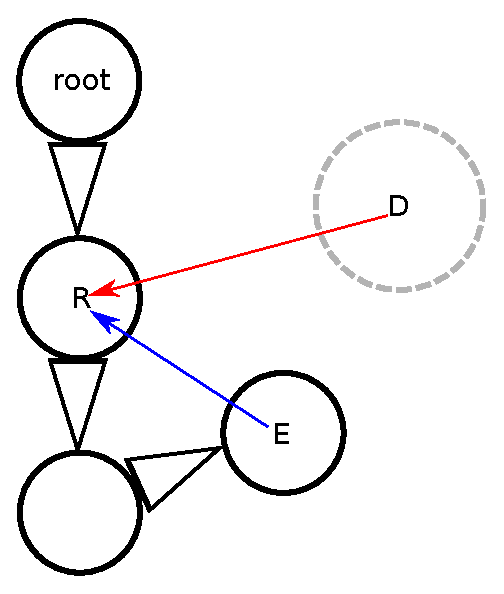
\includegraphics[width=2.5in]{images/ik/ccd.eps}
	\caption[Diagram of the process of CCD Inverse Kinematics]{Depicted is a chain of joints, with a root joint, an end joint E, and two joints in the middle of the chain.  To move the end joint E, which may for example be a hand or foot, to position D, iterate over the chain of joints and calculate the vectors between the current and end joint positions as well as the vector between the current joint position and the destination for the end joint.  The dot product of the normalized vectors then gives the cosine of the angle between these vectors.  Rotating R by this angle will then align the vectors, moving E towards position D.  The dotted gray circle shows an example target area in which the joint E is considered ``close enough'' to position D, allowing the algorithm to terminate if the center of E is anywhere within that circle.  If D is farther away than the total length of the joint chain, the algorithm is set to terminate after a user-specified number of iterations, in our case 30.}
	\label{fig:ccd}
\end{figure}

A solution to the joint positions is found greedily using these constraints, and gradient descent method which works on single-chains of joints.  A single chain of joints is a sequence of joints in which each joint has a single child and a single parent, with one root joint and one leaf joint which lack a parent and child respectively.  This hierarchy may be specified as a subtree of the skeleton in which these conditions hold true, as in our simulation where the joints from the hip to the heel are considered separately for each leg.  Given the hierarchy of joints and a desired position for one of the non-root nodes of the chain, cyclic-coordinate descent (CCD) is used to determine rotations of the joints between the joint in question and the root that will minimize the distance between the joint in question and the desired position as done by Lander \cite{kine1, kine2}.  This algorithm is shown in Algorithm \ref{alg:ik}, with a visual representation of a calculation for a single joint in the chain shown in Figure \ref{fig:ccd}.

\begin{algorithm}[ht]
	\centering
	\begin{algorithmic}[H]
		\Function{SingleChainIK}{C, D, E}
		\Repeat
		\ForAll{Joints R between E and the root, starting with the end E}
			\State $\theta = \cos^{-1} \left(\vec{RD} \cdot \vec{RE}\right)$
			\State Rotate R by $\theta$
		\EndFor
		\Until{\textit{Desired number of iterations performed} or \textbf{E} \textit{is close enough to} \textbf{D}}
		\EndFunction
	\end{algorithmic}
	\caption[Single chain IK algorithm]{Given chain of joints C, move joint E to position D using cyclic coordinate descent.  This process iteratively moves joint E closer to the location D, concentrating on each joint R in the chain one at a time and solving the geometric problem of minimizing distance between E and D by rotating R.  D is the desired position of the body part, such as where the toe should be placed and E is the joint that should be moved to the desired position.  The vectors RD and RE are the vectors between the positions of joints R and E, and joint R and the desired location D in $\mathbb{R}^3$.}
	\label{alg:ik}
\end{algorithm}


This approach is simpler to implement than other approaches such as the pseudo-inverse of the Jacobian for the specific case of single chains of joints.  In addition, this approach allows some flexibility, specifically in constraints of the joints.  As each joint is addressed individually instead of the system as a whole, any constraints placed on the joint can easily be accounted for by simply preventing the joint from rotating out of the desired range while the rest of the system continues to move as close as possible to the solution.  One downside is that a halting condition must be determined, through a minimum acceptable distance.  Additionally, the algorithm does not halt if D is farther from the root position of the chain than the length of the chain, i.e. it is farther away than the length of the limb.  To handle the case where the joint cannot be moved within this minimum distance, a maximum number of iterations must be designated.  In practice, 100 iterations is enough to converge, with as few as 30 working well for our simulation.

%%%%%%%%%%%%%%%%%%%%%%%%%%%%%%%%%%%%%%%%%%%%%%%
%               Torque Method                 %
%%%%%%%%%%%%%%%%%%%%%%%%%%%%%%%%%%%%%%%%%%%%%%%
\section{Torque-Based Simulation}
\label{section:torque}
One method of simulation we attempted used springs placed along the length of each limb to produce a torque on the joints of the character.  Torques on the joints result from the force of the muscle pulling a bone to rotate about the joint, resulting in a complex system of motion with each bone rotating around the joints.  These rotations combine to move the body in a direction, allowing a character's control to be centered around degree and timing of muscle activation. 

Our method for this type of simulation was inspired by the other work in complex muscle based simulation for bipeds such as in Geijtenbeek et al. \cite{muscle_based_bipeds}.  In our case, we take the muscle as constantly activated, which means that its spring constant defines the strength of the muscle, allowing the user to set the activation manually.  This muscle is then stretched to produce the desired torque by bending the affected limb.  The restoring force of the spring-muscles produce torques which are used to calculate angular momentum, and from that linear momentum.  Linear momentum is then used to calculate the resulting acceleration.

\subsection{Calculation of Required Velocity and Acceleration Given Time Constraints}
\label{subsection:torque_path}
%\begin{figure}[ht]
%	\centering
%	\begin{tikzpicture}[node distance=1cm and 1cm, auto]
% Path Estimate Phase
	%	Path Estimate Stage
    \node [stage] (path) {\nodebox{5cm}{Path Estimate \[a = \dfrac{2 (x - x_0 - v_0 t)}{t^2} \]}};
    %	Path Estimate Data
    \node [data, above= of path] (xf) {\nodebox{2cm}{Target Position ($x$)}};
    \node [data, left= of xf] (xi) {\nodebox{2cm}{Initial Position ($x_0$)}};
    \node [data, left= of xi](t) {\nodebox{2cm}{Time ($t$)}};
    \node [data, right= of xf] (vi) {\nodebox{2cm}{Initial Velocity ($v_0$)}};
    \node [data, below= of path] (accel) {\nodebox{3cm}{Target Acceleration ($a$)}};
    
    \path [line] (xi) |- (path);
    \path [line] (xf) -- (path);
    \path [line] (t) |- (path);
    \path [line] (vi) |- (path);
    \path [line] (path) -- (accel);
\end{tikzpicture}
%	\caption[Diagram of path estimation algorithm]{Diagram of the path estimation step.}
%	\label{fig:pathEstimate}
%\end{figure}

%\begin{figure}[ht]
%	\label{fig:pathExample}
%	\caption[Example of estimated path]{Example of a path estimation.}
%\end{figure}
Before calculations relating to the model's skeleton are performed, an initial estimate of the jump path is performed.  The estimate uses a forward kinematic calculation to determine the velocity required to move an object through the air from the initial position of the model to a final position.  This path is specified indirectly by the user by setting time in air, gravity, and desired displacement in three dimensional space, which necessarily describe a parabolic path assuming that displacement and gravity are not 0, and that gravity is an attractive force pulling the character toward the ground.  While perhaps somewhat less intuitive than positioning the character exactly how the artist wants it for each frame, this allows a wide range of physically plausible, simple jumps to be produced.  In such cases, this reduces work excepting special case jumps, such as those found in Warner Brothers' Looney Toons.

The user specifies a desired time ($t_{air}$) that indicates the time the character will spend airborne during the animation, i.e. the time between when the character's feet break contact with the ground and when they regain contact with the ground.  Changes to this time affect the animation length as well as modify the peak height of the jump, as a longer time will necessarily require the character to be airborne longer, and thus be higher in the air.  While this reduces the direct control the artist has, this provides a simple way to control animation length.

The initial velocity is given by a manipulation of a simple kinematic equation \[ \vec{x} = \vec{x_0} + \vec{v_0} t_{air} + \frac{1}{2} \vec{a} t_{air}^2 \] derived from the relationships between acceleration ($\vec{a}$), velocity ($\vec{v}$), and displacement ($\vec{x} - \vec{x_0}$), namely
\begin{align*}
	\vec{v} &= \dfrac{d\vec{x}}{dt} \\
	\vec{a} &= \dfrac{d\vec{v}}{dt}
\end{align*}.

This relationship gives us the velocity, given a known start position ($\vec{x_0}$), destination ($\vec{x}$), acceleration ($\vec{a}$), and time ($t_{air}$).  As this describes the path of the character once it breaks contact with the ground, the time referred to only covers the time between the character breaking contact with the ground and when their feet touch again at the end of the jump  The only force, and therefore acceleration acting upon the character while in the air is gravity, thus giving 
\[ \vec{v_0} = \dfrac{\vec{x} - \vec{x_0}}{t_{air}} - \dfrac{\vec{g}t}{2} \]
to describe the initial velocity our character has upon breaking contact with the ground, which then decays over the course of the jump due to gravity to produce a parabolic path.  The equation considers the character as a point mass traveling in a vacuum, meaning there is no consideration of friction, drag, or rotational movements.  Acceleration can then be determined as 
\begin{align*}
	a &= \dfrac{dv}{dt} \\
	&= \dfrac{\vec{v_f} - \vec{v_i}}{t_{windup}} \\
	&= \dfrac{\vec{v_0} - {v_i}}{t_{windup}}
\end{align*}
where $\vec{v_i}$ is the initial velocity of the character before the jump calculations began.  This accommodates jumps where the character is already moving.

%There is an additional modification to the equation of $\frac{1}{2} g t_{air}$, which considers that the upward velocity of the acceleration is determined by gravity.  Assuming that gravity is a vector with only a vertical component, we can calculate the necessary vertical component for our acceleration by calculating the initial velocity achieved from our calculated acceleration by using the fact that $a = \dfrac{dv}{dt} = \dfrac{v - v_0}{t}$ or $v = v_0 + at$.  By calculating the velocity resulting from the windup, $v = at$ we can substitute this into 

\subsection{Windup Animation of the Character Based on Required Acceleration}
\label{subsection:torque_windup}
%From this force, the acceleration can be determined using $F=ma$ from classical mechanics.  This assumes the character is a rigid body with negligible air resistance acted upon by gravity of $10\frac{m}{s}$.  The mass is calculated as the summed total of the distributed masses assigned to the character's limbs, which are summed to produce a total mass for the character.

Using the calculated velocity and acceleration, we compare the desired values to achieve a particular path with the values produced by the muscles on the skeleton.  To compute a resultant instant linear acceleration, we start from the muscle and calculate the torque resulting from the muscle's contraction.  First we calculate the scalar force of the muscle-spring as $F = -k s$ where $s$ is the spring displacement as calculated in section \ref{subsection:skel_joints}.  Using the scalar force, we calculate the torque and the angular momentum.  Torque magnitude can be calculated as \[\tau = r F\] where $r$ in this case is the scalar distance between the pivot point and the location of force application.  In our case, this is the distance from the center of the joint to the major anchor point, which we consider to be the anchor point highest in the hierarchy, which is the bone most expected to move.  The direction of the torque is the normal vector to the plane of rotation, calculated as the cross product between the directions to each anchor point which gives the plane of rotation about the joint.

Angular momentum is derived from torque, as \[\vec{\tau} = \dfrac{d\vec{L}}{dt}\] where $\vec{\tau}$ is torque and $\vec{L}$ is the angular momentum.  The angular momentum can then be calculated as $\vec{\tau} t_{windup}$.  Angular momentum is used to calculate linear momentum by finding the tangent to the circle at the moment of takeoff.  The magnitude of the linear momentum is then calculated as \[p = \frac{L}{r}\] which then gives the acceleration as follows \[ \vec{a} = \frac{1}{m}\left(\dfrac{d\vec{p}}{dt}\right)\] where m is the mass of the character.

\subsubsection{Sampling of Torque Values at Uniformly Distributed Pelvis Positions}
\label{subsubsection:torque_sample}

In order to determine the position of the character that produces this acceleration, we sample uniformly over a region in which the character is balanced, excluding some points where the character may be balanced in favor of a simpler region.   A sample is described by the position of the pelvis joint, the resulting linear momentum, and a vector describing the displacement of the character's center of mass from the center of its support to indicate balance as described above.  Samples were restricted to a box defined by a rectangle around the character's feet with a height reaching the position of the character's pelvis when standing at rest.  Any sample outside of this volume was assumed to put the character off balance due to the lack of upper body definition in our simulation.

Samples were then taken at uniformly distributed positions in this region.  The calculated acceleration was projected onto the desired acceleration vector through the dot product, with values greater than or equal to the desired acceleration's magnitude indicating a plausible solution.  These plausible solutions are then ordered by their balance error, calculated as the difference in position between the center of mass and the center of the supporting polygon.  The first result of this list is then chosen as the candidate answer and the pelvis is moved towards this sample.  At each iteration this is repeated until the desired acceleration is achieved.  A plot of samples for a particular set of values, in this case all muscle constants set to $k=20000$, is shown in Figure \ref{fig:torque_samples}.  An equation for the described calculation is shown below.

\[
	E_{accel} = \vec{a_{desired}}^2 - \vec{a_{desired}} \cdot \vec{a_{calc}} \le \epsilon \left(\vec{a_{desired}}^2\right)
\]

\begin{figure}[ht]
	\centering
	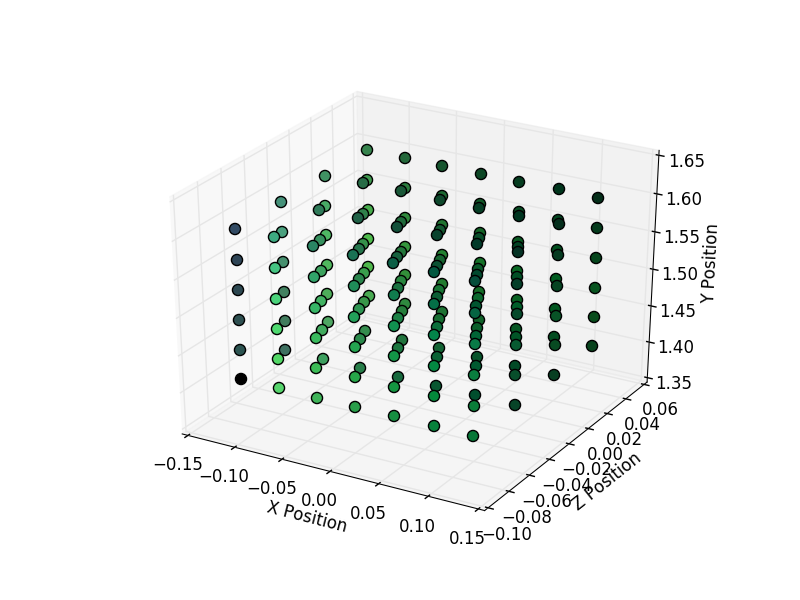
\includegraphics[width=4in]{images/K200000_global_dense_torque.png}
	\caption[A plot of a sample field for the torque based simulation]{A plot of instant linear acceleration samples at different pelvis positions within the balanced region.  The axes shown correspond to the axes of the world, with x, y, and z of the plot corresponding to the x, y, and z position in space.  Color indicates the magnitude, with the red, green, and blue channels corresponding to the x, y, and z components respectively of the acceleration sample.  Lighter color indicates a larger magnitude.  This is a clear example of the failures of this simulation method, as the samples seem to continuously increase from the one corner of the bounding box to the opposite diagonally, which does not produce a plausible animation as the character heavily favors one side, even with symmetric strengths.}
	\label{fig:torque_samples}
\end{figure}

Each iteration the error for the skeleton is calculated by comparing the current state of the skeleton to the desired acceleration and a sample is selected.  If the error is above the tolerance, a new position for the hip is calculated using proportional-derivative control, where the new position for the iteration of the controller, $u(i)$, is calculated as \[u(i) = k_p E_{all}(i - 1) + k_d(E_{all}(i-1) - E_{all}(i-2))\] where $i$ is the iteration, and $k_p$ and $k_d$ are weights which determine the rate of change.  The input to this PD controller is calculated by selecting a sample from the set of samples based on the acceleration error of the sample.  After filtering all plausible candidates from the samples, the candidate which minimizes balance error is selected and the vector between the current pelvis position and the sample pelvis position is given to the PD controller.  

The hip is repositioned based on the output of the PD controller, and the inverse kinematics component then iterates to calculate the positions of the remaining leg joints, assuming the feet should remain in the same position on the ground and the pelvis should remain at the chosen position.  This chooses a solution for the intervening joints.  At the next iteration, these new joint positions and angles are then used to compute the instant linear acceleration, center of mass, balance error, and acceleration error which are then passed back to the PD controller until the error in acceleration is below the tolerance.


\subsection{Extension of the Character's Body and Takeoff from Ground}
\label{subsection:thrust}
Upward acceleration is animated by calculating the angular accelerations of the joints given the forces acting upon them and the resulting torques.  Torque is the change in angular momentum over time, allowing for the acceleration to be calculated as the mass can be assumed to be constant: \[\tau = \dfrac{dL}{dt} = m \dfrac{dv_{\theta}}{dt} = m a_{\theta}\] where $\tau$ is the torque of a joint, $L$ is the angular momentum, $m$ is the mass of the limb, which must take into account the mass of the rest of the body which is also moved by the limb, $v_{\theta}$ is the angular velocity and $a_{\theta}$ is the angular acceleration. This results in the below equation for determining angular acceleration. \[a_{\theta} = \dfrac{\tau}{m}\]

Using angular acceleration, the intermediary poses for the model can be determined at each time step.   For each frame, an explicit Euler integration is performed to determine first angular velocity and finally angle.  As the character continues to extend, a check is made for if the character has yet reached full extension by calculating muscle utilization as described in Section \ref{subsection:skel_joints}.  At full extension, when the limbs are no longer in use, the character can no longer accelerate in the direction of the jump, and the character breaks contact with the ground to enter the in-air phase.

As the windup phase of the torque based simulation fails, it is difficult to quantify or qualify the success and failure of this portion of the simulation.  For values where the simulation could not complete the windup phase, the in-air portion is unavailable and for values where the windup phase completes, the values are erratic and fail to produce valid poses, often resulting in extreme contortions of the model.


%%%%%%%%%%%%%%%%%%%%%%%%%%%%%%%%%%%%%%%
%               Energy                %
%%%%%%%%%%%%%%%%%%%%%%%%%%%%%%%%%%%%%%%
\section{Energy-Based Simulation}
\label{section:energy}
Another way we simulated jumping motions was energy based.  We assumed that the kinetic energy of the character traveling at a calculated velocity from its start position to the destination position is equivalent to the summed elastic potential energies of the leg muscles.  The direction of the velocity is determined by the direction the center of mass is accelerated after the windup phase, and we assume that this is achievable given that the character can achieve the desired energy.  

Change in direction is accomplished through usage of the feet and shift of weight during the acceleration and windup phases, applied through balance and inverse kinematic calculations.  If a character wishes to move forward, they shift their weight back farther during windup, allowing them to accelerate forward farther before becoming airborne.  In the same way, shifting to one side can allow the character to accelerate in the opposite direction for non-forward jumps.  As with the torque-based simulation, the jump follows the stages of path estimation, windup, thrust, in-air, and landing.

\subsection{Path Estimation and Windup}
\label{subsection:energy_path}
Kinetic energy is calculated as \[ E_k = \frac{1}{2} m v^2 \] where $m$ is the mass of the character and $v$ is the velocity.  Mass is a constant specified by the user, and we calculate the desired velocity and acceleration as in the torque based path estimation as described in section \ref{subsection:torque_path}.

Like with the torque-based method, we took samples in the region where the character maintains balance as in section \ref{subsubsection:torque_sample}.  Samples were collected at regular intervals within a bounding box defined by the character's supporting polygon, the ground, and the the height of the character's pelvis at full extension.  The pelvis was repositioned and the resulting elastic potential energy measured.  Candidate samples were selected by finding all samples with \[ E_{kinetic} - E_{elastic} \le \epsilon(E_kinetic)\] and the candidate with the lowest incurred balance error was selected.

\begin{figure}[ht]
	\centering
	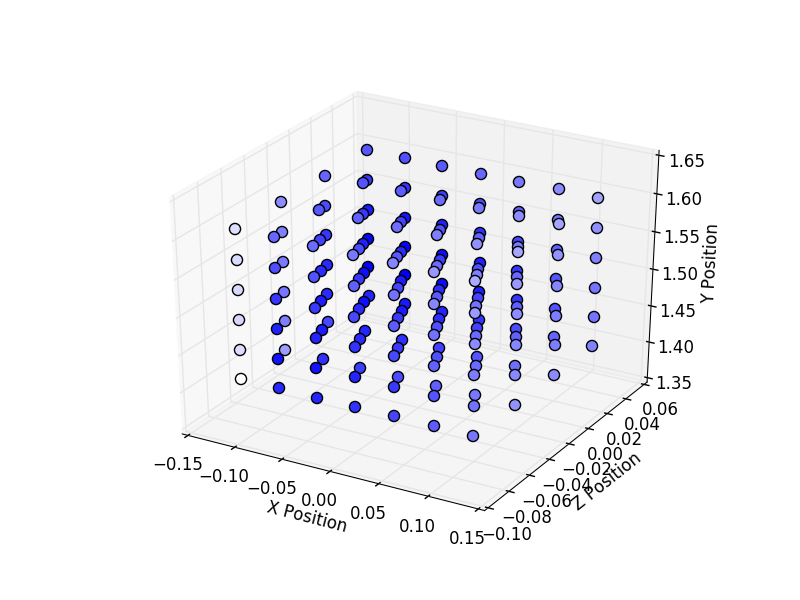
\includegraphics[width=4in]{images/K200000_global_dense.png}
	\caption[A plot of a sample field for energy based simulation]{A graph of samples for the character with all muscle k values set to $20000$.  The pelvis positions are plotted, with the color of the data point indicating the energy.  A darker point indicates a higher total elastic energy calculated for the skeleton when the pelvis is positioned at that point.}
	\label{fig:energy_samples}
\end{figure}

Our sampling method does not guarantee an optimal solution, but can be seen as guaranteeing an approximate minimum.  We choose a sample with minimum balance error and iteratively approach it, which greedily finds the nearest sample to the rest pose which satisfies the energy equivalence, $E_{kinetic} = \displaystyle\sum E_{elastic}$.  While not guaranteed to be the minimum, this guarantees that we find a near-minimum value assuming the region is continuous.  Figure \ref{fig:energy_samples} is a graph of samples for a particular run with all muscle $k$ values set to 20000.  Color indicates the calculated energy for the sample point, with higher saturation of blue indicating a higher energy value for the sample.  The higher energy samples tend to be clustered towards the center of the sample group, which meets expectations as most humans will bend to a position such that their hip is between its normal position when standing and the level of their knees.

Table \ref{tab:force_est} shows examples of estimated values produced by the muscle crossing the knee joint given several different $k$ values over a range of joint angles.  By comparing the summed calculated energy output with the desired, we check if the current pose produces enough elastic energy for the intended motion.

\begin{table}[ht]
	\centering
	\begin{tabular}{| c | c | c | c | c | c | c | c | c | c | c |}
	\hline
	$\mathbf{k}$       & $\mathbf{r}$     & $\mathbf{\theta_{deg}}$ & $\mathbf{\theta_{rad}}$ & $\mathbf{x}$       & $\mathbf{F}$       & $\mathbf{E}$       \\ \hline %& $\sin(\pi - \theta)$  & $\sin\frac{\theta}{2}$    & $\dfrac{\sin(\pi - \theta)}{\sin\frac{\theta}{2}}$  \\ \hline
	200000  & 0.05  & 170            & 2.96           & 0.0087  & 1743.11 & 7.59    \\ \hline %& 0.17                  & 0.9961                    & 0.174311485   \\ \hline
	200000  & 0.05  & 160            & 2.79           & 0.0173  & 3472.96 & 30.15   \\ \hline %& 0.34                  & 0.9848                    & 0.347296355   \\ \hline
	200000  & 0.05  & 150            & 2.61           & 0.0258  & 5176.38 & 66.98   \\ \hline %& 0.5                   & 0.9659                    & 0.51763809    \\ \hline
	200000  & 0.05  & 140            & 2.44           & 0.0342  & 6840.40 & 116.97  \\ \hline %& 0.64                  & 0.9396                    & 0.684040287   \\ \hline
	200000  & 0.05  & 130            & 2.26           & 0.0422  & 8452.36 & 178.60  \\ \hline %& 0.76                  & 0.9063                    & 0.845236523   \\ \hline
	200000  & 0.05  & 120            & 2.09           & 0.05    & 10000   & 250     \\ \hline %& 0.86                  & 0.8660                    & 1             \\ \hline
	200000  & 0.05  & 110            & 1.91           & 0.0573  & 11471.5 & 328.98  \\ \hline %& 0.93                  & 0.8191                    & 1.147152873   \\ \hline
	200000  & 0.05  & 100            & 1.74           & 0.0642  & 12855.7 & 413.17  \\ \hline %& 0.98                  & 0.7660                    & 1.285575219   \\ \hline
	200000  & 0.05  & 90             & 1.57           & 0.0707  & 14142.1 & 500     \\ \hline %& 1                     & 0.7071                    & 1.414213562   \\ \hline
	20000   & 0.05  & 170            & 2.96           & 0.0087  & 174.311 & 0.75    \\ \hline %& 0.17                  & 0.9961                    & 0.174311485   \\ \hline
	20000   & 0.05  & 160            & 2.79           & 0.0173  & 347.296 & 3.01    \\ \hline %& 0.34                  & 0.9848                    & 0.347296355   \\ \hline
	20000   & 0.05  & 150            & 2.61           & 0.0258  & 517.638 & 6.69    \\ \hline %& 0.5                   & 0.9659                    & 0.51763809    \\ \hline
	20000   & 0.05  & 140            & 2.44           & 0.0342  & 684.040 & 11.69   \\ \hline %& 0.64                  & 0.9396                    & 0.684040287   \\ \hline
	20000   & 0.05  & 130            & 2.26           & 0.0422  & 845.236 & 17.86   \\ \hline %& 0.76                  & 0.9063                    & 0.845236523   \\ \hline
	20000   & 0.05  & 120            & 2.09           & 0.05    & 1000    & 25      \\ \hline %& 0.86                  & 0.8660                    & 1             \\ \hline
	20000   & 0.05  & 110            & 1.91           & 0.0573  & 1147.15 & 32.89   \\ \hline %& 0.93                  & 0.8191                    & 1.147152873   \\ \hline
	20000   & 0.05  & 100            & 1.74           & 0.0642  & 1285.57 & 41.31   \\ \hline %& 0.98                  & 0.7660                    & 1.285575219   \\ \hline
	20000   & 0.05  & 90             & 1.57           & 0.0707  & 1414.21 & 50      \\ \hline %& 1                     & 0.7071                    & 1.414213562   \\ \hline
	24000   & 0.05  & 90             & 1.57           & 0.0707  & 1697.05 & 60      \\ \hline %& 1                     & 0.7071                    & 1.414213562   \\ \hline
	16000   & 0.05  & 90             & 1.57           & 0.0707  & 1131.37 & 40      \\ \hline %& 1                     & 0.7071                    & 1.414213562   \\ \hline
	40000   & 0.05  & 90             & 1.57           & 0.0707  & 2828.42 & 100     \\ \hline %& 1                     & 0.7071                    & 1.414213562   \\ \hline
\end{tabular}

	\caption[Table of estimated forces given $k$ values and joint angles]{Above is a table of different displacement (s), force (F), and energy (E) values calculated given a constant bone width of $0.05m$, varying $k$ and varying angle of the joint.  These values are for a single knee, with one muscle crossing the joint.}
	\label{tab:force_est}
\end{table}

%Given that work is the change in kinetic energy, velocity
%\begin{align*}
%	W &= F d \\
%	&= \delta E \\
%	&= \frac{1}{2} m \left(v^2 - v_0^2\right)
%\end{align*}

\subsection{Solutions to the Energy Assignment Problem}
\label{subsection:energy_prob}
The setup of the problem resembles a quadratic programming problem.  In this problem, we minimize: \[ \vec{x}^T \mathbf{Q} \vec{x} \] subject to
\[ \vec{x}^T \mathbf{P} \vec{x} \le r \] where $x \in R^6$ and $\mathbf{Q}$ and $\mathbf{P}$ are square, $6 \times 6$ matrices.  $\mathbf{Q}$ for our problem is a diagonal matrix, where the diagonals contain the spring constants $\left\lbrace k_1, k_2, ... , k_6 \right\rbrace$ and $\mathbf{P}$ is $- \mathbf{Q}$.  We can introduce additional constraints in the form of maximum and minimum values for all $x_i \in \vec{x}$, where the minimum and maximum are calculated at the minimum and maximum rotations of the joint, producing the extremes in spring displacement.

This problem of quadratically constrained quadratic programming is NP-hard and as such we sought a simpler problem or approximation to solve to obtain a solution.  As with the torque method, we choose a sampling-based approach as there is a known limit on the possible solutions in our case: balance.  

\subsection{Thrust, In-Air, and Landing}
\label{subsection:energy_thrust}
Thrust for the energy based simulation works off of explicit euler integration.  The calculated acceleration from the path estimation stage is used to accelerate the character over the duration of $t_{windup}$.  At each time step, the pelvis is translated by $v_{takeoff}$, which begins at 0 and gains $\vec{a} dt$ per frame.  Each frame the character's extension is checked using the function described in section \ref{subsection:skel_joints}, and when it falls below a tolerance of $0.1$, the character is considered fully extended and the in air phase begins.  During the thrust, the movement can sometimes proceed faster than the IK solver can converge, so we pause the simulation briefly and only iterate the solver until it converges.

The in air phase proceeds similarly, with the character translated by the calculated velocity from the path estimate each frame.  Velocity is modified by $\vec{g} dt$ where $\vec{g}$ is the acceleration due to gravity, resulting in the desired parabolic path of the player through the air.  Ray casts are performed to check if the character's feet have contacted a surface to land on.  A ray cast is used instead of the collision detection of a capsule collider as is normally used for physics interactions with characters in \unity as it provides more information about the distance from surfaces.  This allows the prevention of intersection errors where the rougher shape of the collider, which is usually a box, sphere or capsule, causes the character to fail to collide properly and intersects a shape.  Performing per-triangle collision would also solve this issue, but as characters are expected to contain tens of thousands of triangles.  These ray casts are made from above toe, heel, and middle of the foot, starting above and passing through the points to produce a longer ray for more stable results.  Once one of these ray casts indicates the feet have touched such a surface, the character enters the landing phase.

A landing controller is beyond the scope of this thesis, and thus we end the simulation as the character's feet touch a suitable surface.  As described in chapter \ref{chapter:previous_work}, other controllers can be composed with this controller to produce a full animation, handling the complexities of the landing motion as a separate, modular controller.

\section{Summary}
\label{subsection:animation_summary}
The character is modeled as a mesh with a skeleton and muscles.   The skeleton was created as a tree of joints with the root at the hip.  Muscles were placed along the limbs, crossing a single joint and anchored to the bones on either side.  Force and energy outputs of the muscles were calculated as linear springs, with spring displacements calculated from the angle of the joint.  An inverse kinematic solver was used to aid in creating poses.

Two methods were used for the simulation, one using torque based calculations and the other using energy based calculations.  Each method proceeded through the stages of path estimate, windup, thrust, in air, and landing, with similar calculations used to produce an error function to quantify character poses.  In the torque based simulation, error was calculated by using the muscles to calculate torques, and from the torques accelerations.  In the energy based simulation, error was calculated as the difference between elastic potential energy and target kinetic energy.  

Samples were collected using these error functions, with the selected best sample minimizing both the balance error and either the acceleration or energy errors for the torque and energy simulations respectively.  A PD controller iteratively moved the character's pelvis position towards the selected sample until the error between the calculated values for the frame and the desired values were below a tolerance.  After the character moved its pelvis to the chosen sample position to reduce the error below tolerance, it performed the thrust and in air portions of the jump treated as a rigid body, with the simulation ending when the character's feet touch the ground.